\subsection{What Is Compared}
\label{sec:comparisons}
A \emph{setting} is one task under one visual variant, for example one camera viewpoint. Every comparison runs a setting twice, clean and perturbed, from the same initial physical state and with the same policy noise, so that only the image differs. The two runs share a state only at the first query, where responses and commands are compared; motion is compared after 5 and 60 controls, and task success at the end of the episode.

Internal recordings and paired executions cover the same 268 settings on 40 tasks, in separate episodes. Primary comparisons use the 202 settings to which LIBERO-Plus assigns a difficulty level, on the 28 tasks that have all four families. The settings are a subset of LIBERO-Plus that we chose deliberately: recording internal states and running five executions per setting made the full benchmark impractical, and we left out settings whose perturbation we judged too large for a controlled comparison with the clean run, above all large camera displacements. The labelled settings span all five LIBERO-Plus difficulty levels. Success rates on this panel should not be compared with full-benchmark figures: for $\pi_0$ they are close under Background and Sensor Noise (85.7\% and 78.6\%, against 81.4\% and 79.0\%) but much higher under Camera (66.1\% against 13.8\%)~\cite{fei2026liberoplus}. Each setting is run under two draws of policy noise; one setting under one draw is a \emph{pair} (a \emph{case} in the restoration study), so the recordings give 404 pairs. The restoration study splits the 40 tasks into 9 used to develop it and 31 held out to test it (Sec.~\ref{sec:restoration}; Fig.~\ref{fig:model-measurement}c).

The paired executions run each policy five times per setting (Fig.~\ref{fig:model-measurement}d): two clean runs with different policy noise, two perturbed runs that each share the noise of one clean run, and a repeat of the first clean run, which checks that runs are reproducible. A perturbed run is always compared with the clean run that shares its noise. The two clean runs differ only in their policy noise, so their difference shows how much motion and outcomes vary without any perturbation. We use it as the reference for a perturbation's effect and call the second clean run a \emph{clean rerun}.

\begin{figure*}[t]
\centering
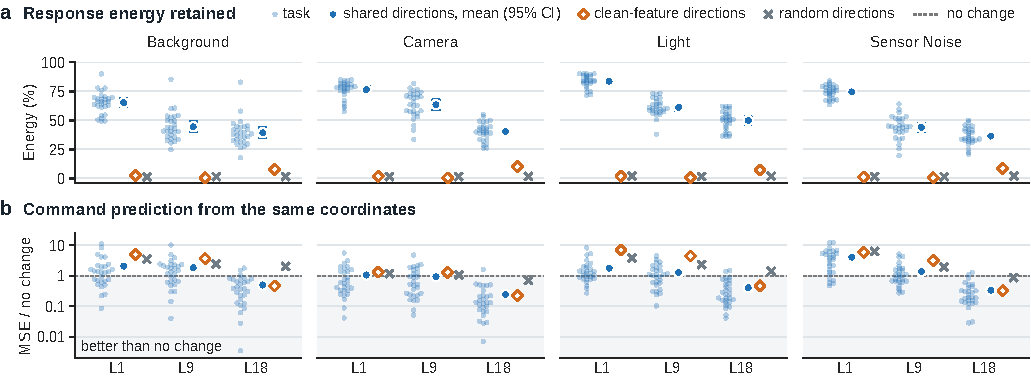
\includegraphics[width=\textwidth]{revised_figures/figure3_geometry_v3.pdf}
\caption{\textbf{Shared directions retain far more of an unseen response than the controls; the commands are predicted best at the last layer.} Both panels: 404 pairs on 28 tasks; each fit leaves out the test tasks and the test family. For the shared directions, small dots are tasks and large dots their means; diamonds and crosses are the two controls. (a) Share of the response energy that 16 directions retain; the means carry pointwise 95\% intervals. (b) Error of a linear readout that predicts the change in the first five commands from the same 16 coordinates, divided by the family-mean error of predicting that the commands do not change; large markers are ratios of task means. Below 1 (shaded), the readout beats predicting no change. Paired comparisons: Supplement, Secs.~S3.4 and~S14.}
\label{fig:token-structure}
\end{figure*}


All averages weight tasks equally, and intervals resample whole tasks. Of the 2,680 planned outcomes of the paired executions, 39 are missing (technical failures or failed validation); on the 28 common tasks they affect only Light. We keep them in the denominator and report bounds (Supplement, Secs.~S1, S5, and~S6).
